
\begin{frame}
	\frametitle{Outline}

	\begin{itemize}
		\item Terminology and introducing incremental classification
		\item Trivia games as an instance of incremental classification
		\item Crowdsourcing incremental classification
		\iflong
			\item Improving venerable machine learning problems
		\fi
		\item New machine learning algorithms to do incremental
                  classification
                  \item Why you should think about using these data?
	\end{itemize}
\end{frame}


\begin{frame}
	\frametitle{\sout{Batch} Rapacious Machine Learning}

	\begin{itemize}
		\item Machine learning typically learns a mapping $f(x) \mapsto y$
		\item Minimizes estimate of the error
		\item {\bf Rapacious} looks at all of $x$
		\item Can we be more selective?
		\begin{itemize}
			\item Annotators (usually) only provide mapping, not their process
			\item Doesn't care how difficult it is to extract features
		\end{itemize}
                \iflong
		\pause
		\item Alternative: asking annotators directly for relevant
                  features~\cite{zaidan-08}
                  \fi
	\end{itemize}
\end{frame}



\begin{frame}
	\frametitle{Approaches}

	\begin{itemize}
		\item Incremental classification
			\begin{itemize}
				\item $x$ is revealed piece by piece
				\item Algorithm gives answer when it wants
				\item \emph{Last} observed part of $x$ usually important / useful
			\end{itemize}
		\item Learning incremental classification when costs are known via decision trees~\cite{norton-89,nunez-91,turney-95,davis-06} or Markov decision process~\cite{zubek-02,ji-07}
		\item In contrast we're going to focus on a problem whose structure is inherently incremental
	\end{itemize}
\end{frame}

\section{Quiz Bowl}

\begin{frame}
	\frametitle{Humans doing Incremental Classification}
	\begin{columns}

	\column{.5\linewidth}
	\begin{itemize}
		\item Game called ``quiz bowl''
		\item Two teams play each other
		\begin{itemize}
			\item Moderator reads a question
			\item When a team knows the answer, they signal (``buzz'' in)
			\item If right, they get points; otherwise, rest of the question is read to the other team
		\end{itemize}
		\item Hundreds of teams in the US alone
                \only<2>{\item Example \dots}
	\end{itemize}

	\column{.5\linewidth}
	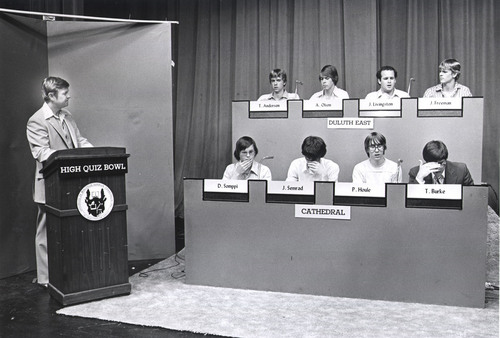
\includegraphics{qb/quizbowl}

	\end{columns}

\end{frame}

\begin{comment}

\begin{frame}[t]
	\frametitle{Sample Question 1}

With Leo Szilard, he invented a doubly-eponymous \only<2->{refrigerator with no moving parts. He did not take interaction with neighbors into account when formulating his theory of} \only<3->{heat capacity, so} \only<4->{Debye adjusted the theory for low temperatures. His} \only<4->{summation convention automatically sums repeated indices in tensor products. His name is attached to the A and B coefficients} \only<5->{for spontaneous and stimulated emission, the subject of one of his multiple groundbreaking 1905 papers. He further developed the model of statistics sent to him by} \only<6->{Bose to describe particles with integer spin. For 10 points, who is this German physicist best known for formulating the} \only<7->{special and general theories of relativity?} \\
\vspace{1cm}
\only<8->{ {\bf Albert \underline{Einstein}}}
\end{frame}

\end{comment}


\begin{frame}[t]
\frametitle{Sample Question}

One is Monte Carlo if at least half of the possible results for all x in a
\only<2->{language it says ``yes'' and ``no'' otherwise. One is called} \only<3->{unambiguous if for any $x$�there is at most one accepting computation. One is
called} \only<4->{oblivious if the position of the} \only<5->{cursor at the $t^{th}$
step depends only on the $t$ and the length of the input. One is} \only<6->{non-deterministic if its sets of next} \only<7->{states may contain more than one
element. For ten points, identify this model of} \only<8->{computation named for
an} \only<9->{English computer scientist.} \\
\only<10->{{\bf ANSWER: \underline{Turing} Machine (prompt on TM)}}


\end{frame}


\begin{frame}[t]
	\frametitle{Sample Question}
A letter from Vergnaud to Chomsky first made the argument that all \only<2->{DPs must have it.  Chomsky called IPs} \only<3->{faulty because its assignment in sentences with verbs like} \only<4->{``believe'' can change the specifier in a process called its} \only<5->{``exceptional marking''.  In Russian, the ending for the} \only<6->{instrumental one is} \only<7->{``om,'' and in German,} \only<8->{``des'' is an article for the genitive one.  For 10 points, name this} \only<9->{linguistic feature that signifies whether a noun is a} \only<10->{subject when it's nominative or an object when it's accusative.} \\
\vspace{.5cm}
\only<11->{ {\bf abstract \underline{case}}}

\only<12->{
  \begin{block}{Things to note}
    \begin{itemize}
    \item Pyramidality
      \iflong
    \item ``For ten points'' (FTP)
      \fi
      \end{itemize}
  \end{block}
}

\end{frame}

\begin{frame}
	\frametitle{Humans doing Incremental Classification}

	\begin{columns}
		\column{.5\linewidth}

		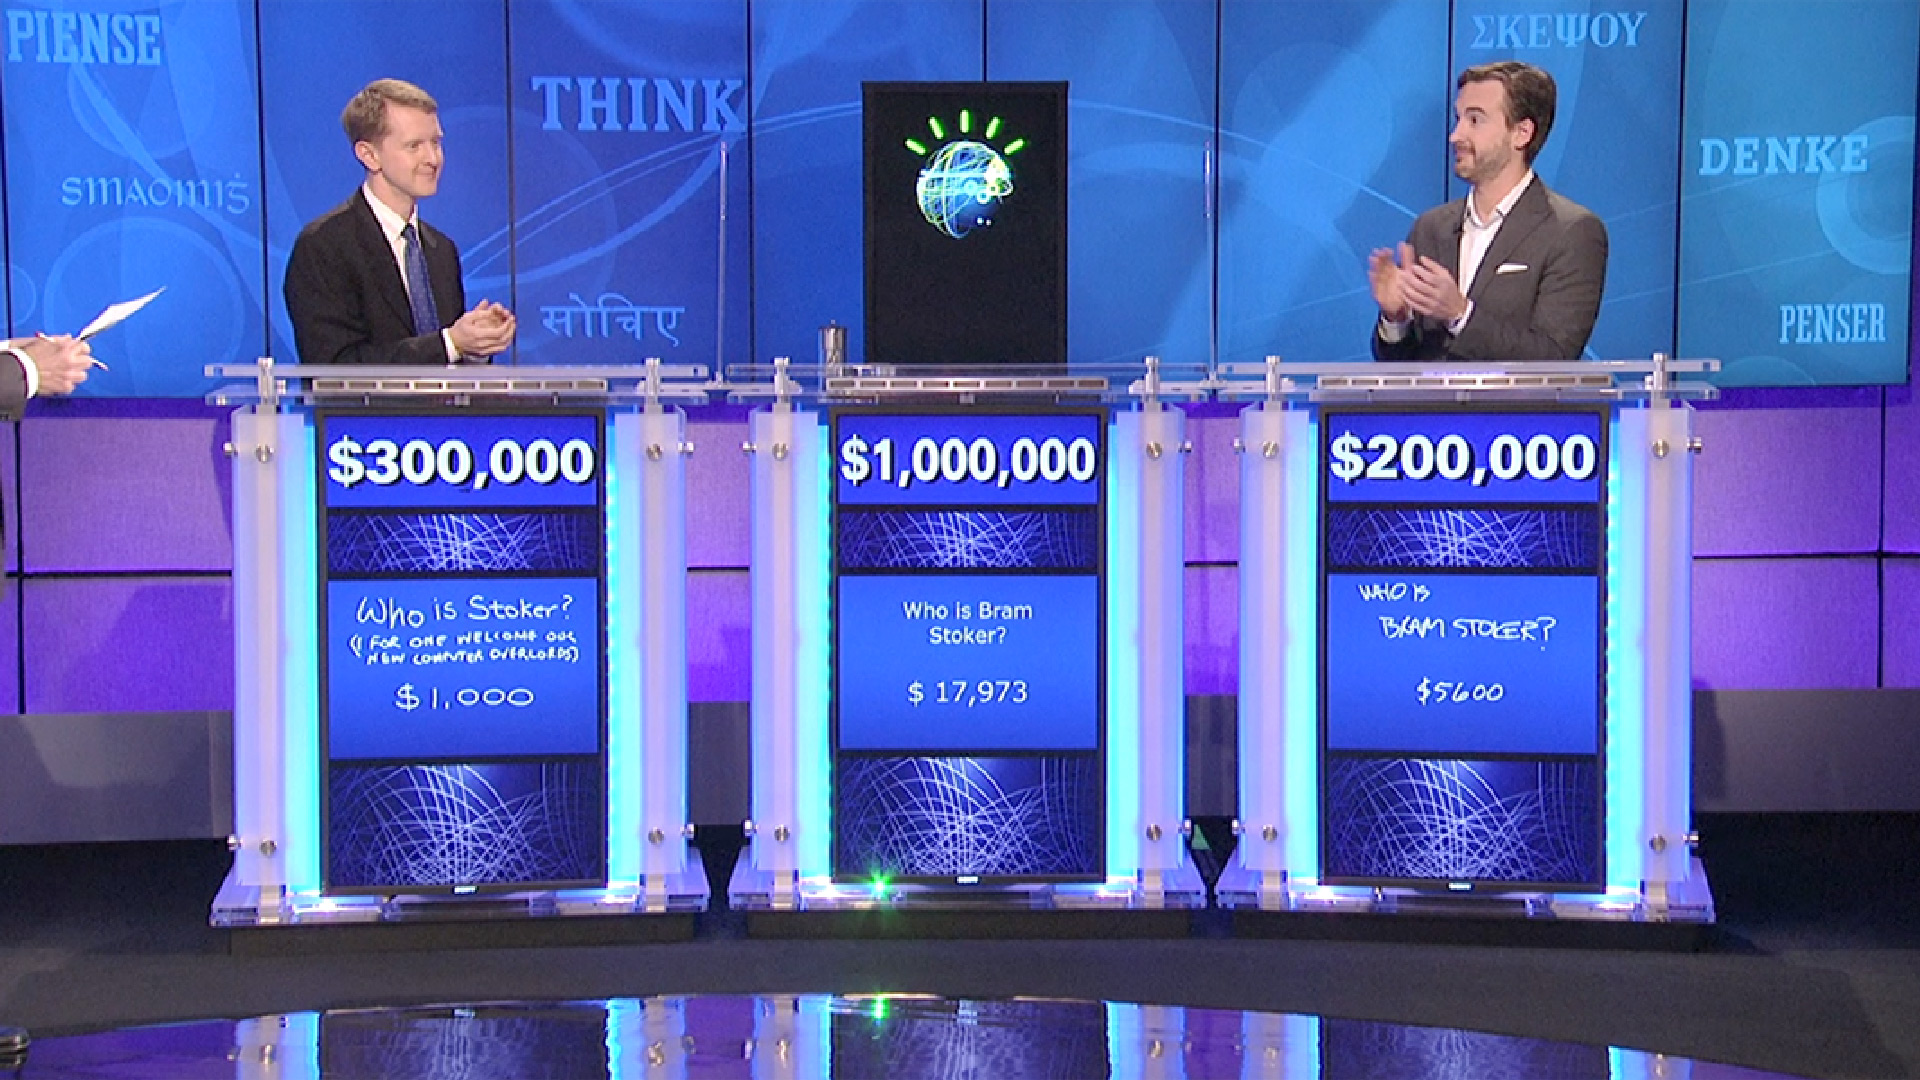
\includegraphics[width=1.0\linewidth]{qb/jeopardy}


		\column{.5\linewidth}
		\begin{itemize}
			\item This is {\bf not} Jeopardy \cite{ferruci-10}
			\item There are buzzers, but players can only buzz at the end of a question
			\item Doesn't discriminate knowledge
			\item Quiz bowl questions are pyramidal
		\end{itemize}

	\end{columns}

\end{frame}



\begin{frame}
	\frametitle{Humans doing Incremental Classification}

	\begin{itemize}
		\item Thousands of questions are written every year
		\item Large question databases
		\item Teams practice on these questions (some online, e.g. IRC)
		\item How can we use this process?
	\end{itemize}

\end{frame}


\section{Data Collection}

\begin{frame}

\frametitle{Interface}

\begin{columns}

	\column{0.5\linewidth}

	\begin{center}
		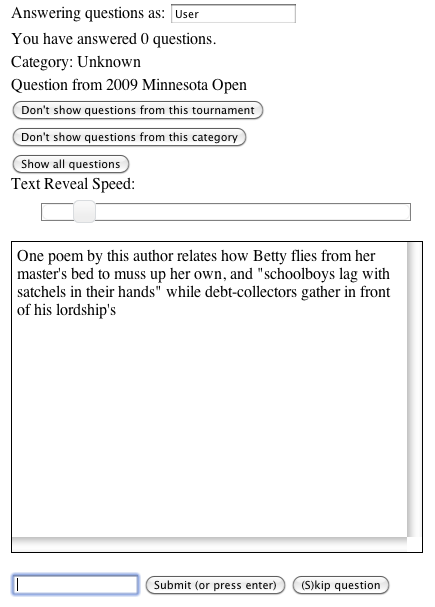
\includegraphics[width=0.9\linewidth]{qb/screenshot}
	\end{center}

	\column{0.5\linewidth}
	\only<1>{
	\begin{itemize}
		\item Users could ``veto'' categories or tournaments
		\item Questions presented in canonical order
		\item Approximate string matching (w/ override)
	\end{itemize}
	}

	\only<2>{
	\begin{itemize}
		\item Started on Amazon Mechanical Turk
		\item 7000 questions were answered in the first day
		\item Over 43000 questions were answered in the space of two weeks
		\item Total of 461 unique users
		\item Leaderboard to encourage users
	\end{itemize}
	}

\end{columns}
\end{frame}

\iflong

\begin{frame}
	\frametitle{Accuracy vs. Speed}

	\begin{center}
	  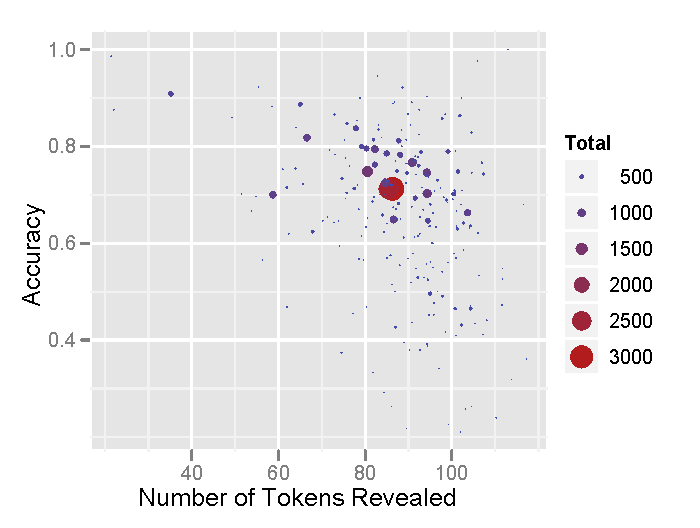
\includegraphics[width=0.9\linewidth]{qb/accuracy_vs_speed}
	  \end{center}

\end{frame}

\fi

\begin{frame}
	\begin{center}

\vspace{-.6cm}
\begin{figure}[tb]
\centering
\iflong
\subfigure[Buzzes over all Questions]{
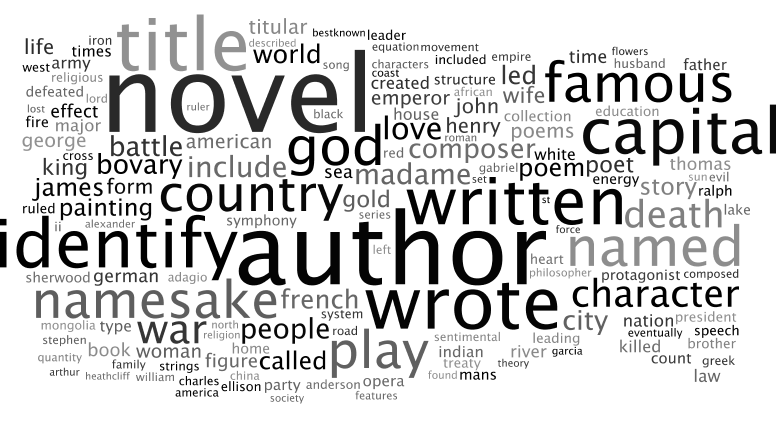
\includegraphics[width=0.6\linewidth]{qb/buzz_cloud}
\label{fig:buzz_cloud}
}
\fi
\subfigure[Wuthering Heights Question Text]{
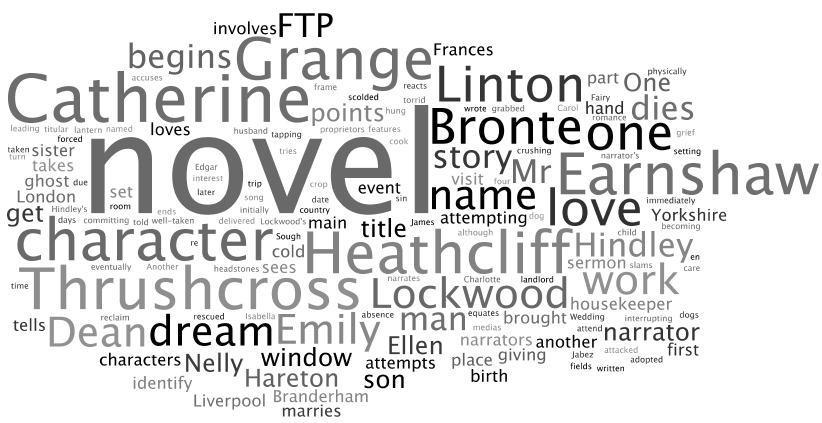
\includegraphics[width=0.45\linewidth]{qb/wuthering_heights_question}
\label{fig:wh_question}
}
\subfigure[Buzzes on Wuthering Heights]{
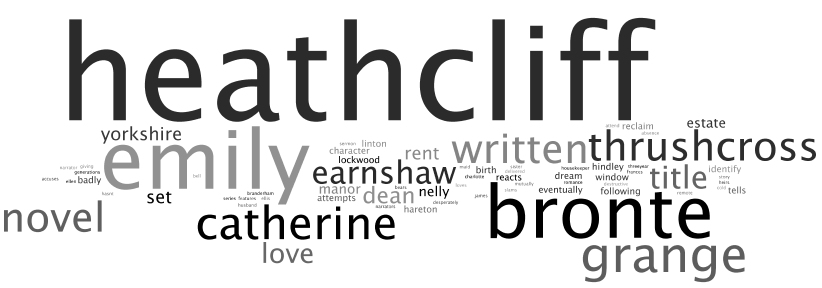
\includegraphics[width=0.45\linewidth]{qb/wuthering_heights_buzz}
\label{fig:wh_buzz}
}
\end{figure}


	\end{center}

\end{frame}
